\documentclass[modern,linenumbers,trackchanges]{aastex7}
%\usepackage{sansmath}
%\sansmath


\usepackage{amsmath} 
\usepackage{color}
\definecolor{black}{rgb}{0,0,0}
\definecolor{blue}{rgb}{0.2,0.2,0.81}
\definecolor{orange}{rgb}{0.92,0.33,0.16}

\definecolor{gray}{rgb}{.5,0.5,0.5}
\newcommand{\todo}[1]{{\color{orange}  #1 \normalfont}}
\newcommand{\zkbt}[1]{{\color{black} #1}\normalfont}
		
\begin{document}
%\title{The Slope of the Cosmic Shoreline is Terrifically Uncertain}
%\title{The Cosmic Shoreline is 3D}
%\title{The Cosmic Shoreline in 3D}
%\title{The Cosmic Shoreline is 3D}
\title{The 3D Cosmic Shoreline for Nurturing Planetary Atmospheres}
%sustaining? preserving? 

\shorttitle{Probabilistic Cosmic Shorelines}


\author[orcid=0000-0002-3321-4924,sname='Berta-Thompson']{Zach K. Berta-Thompson}
\affiliation{University of Colorado Boulder, Department of Astrophysical and Planetary Sciences}
\email[show]{zach.bertathompson@colorado.edu}  


\author[orcid=0000-0001-6484-7559,sname='Wachiraphan']{Patcharapol Wachiraphan}
\affiliation{University of Colorado Boulder, Department of Astrophysical and Planetary Sciences}
\email{patcharapol.wachiraphan@colorado.edu}  



\author[orcid=0000-0001-8504-5862,sname='Murray']{Catriona Murray}
\affiliation{University of Colorado Boulder, Department of Astrophysical and Planetary Sciences}
\email{catriona.murray@colorado.edu}  



% basic parameters for any
\newcommand{\lnw}{-1.39 \pm 0.33}
\newcommand{\logfo}{2.52_{-0.29}^{+0.44}}
\newcommand{\p}{5.79_{-0.41}^{+0.59}}
\newcommand{\q}{1.06_{-0.19}^{+0.27}}
\newcommand{\w}{0.248_{-0.068}^{+0.099}}
\newcommand{\logLnohz}{-2.38_{-0.29}^{+0.23}}
\newcommand{\Lnohz}{0.004_{-0.002}^{+0.003}}



\newcommand{\mrb}{0.041 \pm 0.034}
\newcommand{\mrbsigma}{-1.05 \pm 0.1}
\newcommand{\mrm}{3.38 \pm 0.029}
\newcommand{\mrmsigma}{-0.178 \pm 0.036}

% where HZ + atmospheres intersect
\newcommand{\hzlum}{?}
\newcommand{\hzmass}{?}
\newcommand{\hztype}{?}

\begin{abstract}

Various ``cosmic shorelines" have been proposed to distinguish which planets have atmospheres planets. The fates of individual planet atmospheres may be set by a complex sea of growth and loss processes, driven by unmeasurable environmental factors or unknown historical events. Yet, defining population-level boundaries may help illuminate which processes matter most and identify high-priority targets for future atmospheric searches. Here, we provide a statistical framework for inferring the position, shape, and fuzziness of an instellation-based cosmic shoreline, defined in the three-dimensional space of planet escape velocity, planet bolometric flux received, and host star luminosity; explicitly including luminosity partially circumvents the need to estimate host stars' historical X-ray and ultraviolet fluences. Using Solar System and exoplanet atmospheric constraints, under the restrictive assumption that one planar boundary applies across a wide parameter space, we find the critical flux threshold for atmospheres scales with escape velocity with a power-law index of $p=\p$, steeper than the canonical literature slope of $p=4$, and scales with stellar luminosity with a power-law index of $q=\q$, steep enough to disfavor atmospheres on Earth-sized planets out to the habitable zone for stars less luminous than $\log_{10} (L_\star/L_\sun) = \logLnohz$ (roughly spectral type M4.5V). If we relax the assumption that one power law must stretch from the hottest exoplanets to the coolest Solar System worlds, the narrower question of ``Which warm planets have thick CO$_2$ secondary atmospheres?" is still poorly constrained by data but should improve significantly with planned JWST observations. 

\end{abstract}

\keywords{\uat{Exoplanets}{498}, \uat{Planetary science}{1255}, \uat{Exoplanet astronomy}{486}, \uat{Exoplanet atmospheres}{487}, \uat{Planetary atmospheres}{1244}, \uat{Atmospheric evolution}{2301}, \uat{Planetary climates}{2184}}


\section{Introduction} 
\label{s:introduction}

Where can atmospheres thrive? This question has grown more urgent as astronomers branch out from the Solar System to exoplanets, where atmospheres require great observational expense to measure or sometimes can only be imagined. A complete, precise, and predictive answer to this question might not exist, as each individual atmosphere is the integrated balance of difficult-to-model sources and sinks. Atmospheres grow through early accretion from primordial nebulae, through later impact delivery, through continual magmatic outgassing from the interior, and through evaporation or sublimation of surface volatiles. Atmospheres wither through myriad upper-atmosphere escape processes driven by stellar radiation, stellar winds, and/or impacts; through sequestering into the interior; and through condensation or deposition to the surface. These processes continuously interact with each other, they operate on timescales spanning minutes to gigayears, and they depend on historical environmental inputs that can be wildly uncertain, chaotic, or stochastic. On Earth and other inhabited planets, atmospheric evolution is further complicated by biogeochemical cycles that may include the influence of technological civilizations. For more detail, see reviews by \citet{johnsonExospheresAtmosphericEscape2008, lammerAtmosphericEscapeEvolution2008, tianAtmosphericEscapeSolar2015b, owenAtmosphericEscapeEvolution2019a,  gronoffAtmosphericEscapeProcesses2020, wordsworthAtmospheresRockyExoplanets2022} and textbooks by \citet{chamberlainTheoryPlanetaryAtmospheres1987, pierrehumbertPrinciplesPlanetaryClimate2010, seagerExoplanetAtmospheresPhysical2010, ingersollPlanetaryClimates2013, tianAtmosphericEscapeSolar2015a, lissauerFundamentalPlanetaryScience2019}.
 
Despite the incredible specifics needed to model an atmosphere's detailed history, we can still seek systematic trends among basic planet properties that may allow for the cultivation of an atmosphere. \citet[][hereafter ZC17]{zahnleCosmicShorelineEvidence2017a} distilled this idea into the search for a ``cosmic shoreline'', with dry volatile-poor atmosphere-less worlds (the sand) on one side of the shoreline and worlds rich in volatiles or atmospheres on the other (the lake/sea/ocean). ZC17 explored log-linear boundaries in 2D spaces defined by the planetary escape velocity $v_{\sf esc}$ as a tracer of how strongly planets hold onto volatiles (or various combinations of $v_{\sf esc}$ with planet mass $M$, radius $R$, density $\rho$) and various sources of incoming energy available to drive escape: the current bolometric flux\footnote{In this work we primarily use ``flux'' ($f$) to refer to the power per unit area (W/m$^2$) a planet receives from its star. It is equivalent to ``insolation'' (\underline{in}coming \underline{sol}ar radi\underline{ation}) as used by ZC17, ``instellation'' (\underline{in}coming \underline{stell}ar radi\underline{ation}) introduced for exoplanets by \citet{shieldsEffectHostStar2013}, or ``irradiance.''}
planets receive $f$, the cumulative X-ray and ultraviolet (XUV) fluence planets have received over their history $F_{\sf XUV} = \int_{0}^{\sf now}f_{\sf XUV}(t) dt$, or the estimated velocity of giant impacts $v_{\sf imp}$. Although it is typically less than 0.01\% of a star's bolometric luminous output \citep{franceMUSCLESTreasurySurvey2016}, the difficult-to-measure XUV flux is distinctly important because it drives the upper atmosphere heating and ionization that mediate many escape processes \citep{linskyInferringIntrinsicStellar2024}. ZC17 identified $f \propto v_{\sf esc}^4$ and $F_{\sf XUV} \propto v_{\sf esc}^4$ as effective definitions of instellation-based cosmic shorelines, as well as $v_{\sf imp}/v_{\sf esc} = 5$ as a potential impact-driven shoreline \citep[see also][]{zahnleOriginsAtmospheres1998}.

The ZC17 instellation-based shorelines have been adopted among the exoplanet community trying to identify rocky exoplanets most likely to have atmospheres and to contextualize non-detections of such atmospheres from JWST \citep[][and references therein]{parkcoyPopulationlevelHypothesisTesting2024}. The Rocky Worlds STScI Director's Discretionary Time program is using 500 hours of JWST time to survey terrestrial transiting exoplanets for atmospheres \citep{redfieldReportWorkingGroup2024} and includes estimated location relative to the $F_{\sf XUV}$ shoreline as a metric for target prioritization\footnote{\href{https://rockyworlds.stsci.edu/}{rockyworlds.stsci.edu}}. Since the shoreline is being used, we want to help make it as useful as possible. 

In this work, we revisit the ZC17's instellation-based shorelines through the lens of Bayesian probabilistic modeling. We define a generative model for the probability of a planet having an atmosphere and use it to infer the location, slope, and width of a cosmic shoreline, along with uncertainties on these quantities. We expand the shoreline into 3D, using planetary escape velocity $v_{\sf esc}$, planetary bolometric flux $f$, and stellar luminosity $L_\star$ as three predictors for whether planets have atmospheres. The inclusion of stellar luminosity is designed to remove the need for star-by-star estimates of hard-to-measure environmental drivers for atmospheric escape (like high-energy fluence $F_{\sf XUV}$), moving them to where they can be modeled and marginalized more easily on an ensemble level. We show how to include uncertainties on planet properties in modeling the shoreline and the small effect they have on the actual shoreline parameters. Acknowledging that a true underlying cosmic shoreline is likely crinkled with fjords and peninsulas, tidepools and islands, we apply this approximate model to explore the threshold for atmospheres on both a global scale (from hot transiting exoplanets to the outer edges of the Solar System as in ZC17) and local scale (only planets with solid surfaces and CO$_2$ likely to be in the gas phase) relevant to JWST's current detection capabilities and to habitability.

We assemble planet populations to analyze in \S\ref{s:data}, present the probability model and fitting methodology in \S\ref{s:fitting},  show the inferred shorelines in \S\ref{s:shorelines}, interpret the implications of the derived slopes in \S\ref{s:slopes}, and conclude in \S\ref{s:conclusions}. Code to reproduce all plots in the paper and calculations are include throughout (\href{https://github.com/zkbt/shoreline}{\texttt{</>}}).

\section{Curating the Data}
\label{s:data}

We assemble planetary properties using \texttt{exoatlas} \citep{berta-thompsonZkbtExoatlas2025}. Solar System data come from JPL Solar System Dynamics tables of major planets, dwarf planets, minor planets, and moons\footnote{\href{https://ssd.jpl.nasa.gov}{ssd.jpl.nasa.gov}}. Exoplanet data come from the NASA Exoplanet Archive's \citep{christiansenNASAExoplanetArchive2025}\footnote{\href{https://exoplanetarchive.ipac.caltech.edu}{exoplanetarchive.ipac.caltech.edu}} Planetary Systems Composite Parameters table, which aims to provide as many properties as possible for each planet, sometimes combining values from independent and possibly inconsistent literature sources. For some planets, we noticed significant problems with the chosen parameter combinations and used \texttt{exoatlas} to update the choice of references used. All quantities have units attached with \texttt{astropy.units}, as well as uncertainties propagated through any calculations with numerical samples using \texttt{astropy.uncertainty}. %In \texttt{exoatlas}, missing planet parameters are calculated from other available measurements. 


\subsection{What quantities do we use to predict atmospheres?}

For stellar luminosity $L_\star$, if not present in the raw table, \texttt{exoatlas} calculates it from stellar effective temperature $T_{\sf eff, \star}$ and stellar radius $R_\star$. For the average bolometric flux a planet receives $f = L_\star/(4\pi a^2)$, we first attempt to pull planet semimajor axis $a$ from the table, then second we attempt to calculate it from the orbital period $P$ and stellar mass $M_\star$ via $P^2 = 4\pi^2 a^3/GM_\star$, and then third if necessary from a transit-derived scaled semimajor axis ratio $a/R_\star$. For the gravitational escape velocity of the planet $v_{\sf esc}$, where measurements are available we calculate it as $v_{\sf esc} = \sqrt{2GM / R}$. However, many objects have radii but no measured masses, with radial velocity wobbles or transit-timing variations too weak to detect (transiting planets) or no orbiting bodies to provide dynamical masses (small Solar System objects). 

To be able to include objects without measured masses in our analysis, we derive an empirical radius-to-mass relation from rocky objects with measured masses and radii. We limit to radii smaller than $1.8 {\rm R_\earth}$, as these are likely to be mostly terrestrial \citep{fultonCaliforniaKeplerSurveyVII2018, zengNewPerspectivesExoplanet2021, rogersMostSuperEarthsHave2025}. We fit a linear model $y = m\cdot x + b$ where we define $x_i = \ln (R_i/R_\earth)$ and $y_i = \ln (M_i/M_\earth)$, corresponding to a power-law relationship $M = CR^m$ where $C = e^b$. In addition to the measurement uncertainties on the data $\sigma_{x,i} = \sigma_{\ln R_i} = \sigma_{R_i}/{R_i}$ and $ \sigma_{y_i} =  \sigma_{\ln M_i} =  \sigma_{M,i}/M_i$, we include an intrinsic scatter on the relation $\sigma_{y}$. We allow this intrinsic scatter to vary with radius as $\ln \sigma_{y} = m_\sigma \cdot x + b_\sigma$ to capture the diversity of densities that grows toward very small objects due to effects of composition, structure, and porosity. We infer the parameters of this model ($m$, $b$, $m_\sigma$, $b_\sigma$) following a blog post by \citet[][see also \citealt{hoggDataAnalysisRecipes2010a}]{foreman-mackeyFittingPlaneData2017} with a Gaussian likelihood that analytically marginalizes over the uncertainties in both $x$ and $y$ and an uninformative prior on the slopes $P(m) \propto (1+m^2)^{-3/2}$ as in \citet{vanderplasFrequentismBayesianismPythondriven2014a}. We sample the posterior using \texttt{numpyro} \citep{phanComposableEffectsFlexible2019} with the No U-Turns Sampler \citep[NUTS;][]{hoffmanNoUTurnSamplerAdaptively2011}, using 4 chains each with 5,000 warm-up steps and 50,000 samples, reaching an \citet{gelmanInferenceIterativeSimulation1992} statistic of $\hat{R}=1.0$ and a bulk effective sample size $>10,000$ \citep[][see also \citealt{hoggDataAnalysisRecipes2018}]{vehtariRankNormalizationFoldingLocalization2021} for all parameters. Figure \ref{f:mass-radius} shows the result. The inferred slope of $m = \mrm $ is slightly steeper than a constant density ($m=3$) as expected due to self-gravity more strongly compressing larger planets, and the intercept $b = \mrb$ is close to Earth-like ($b=0$). For the intrinsic scatter, the slope $m_\sigma = \mrmsigma $ and intercept $b_\sigma = \mrbsigma$ imply a 35\% scatter at 1 ${\rm R_\earth}$ that grows to 120\% scatter at $10^{-3}$ ${\rm R_\earth}$. We incorporate the sample means and covariance matrix (which describe the nearly multivariate normal posterior well) into \texttt{exoatlas} to calculate mass estimates with uncertainties that include the uncertainties on the parameters themselves, the intrinsic scatter, and the input radius uncertainties. This relation is valid only for planets without gaseous envelopes contributing significantly to their overall size.

\begin{figure*}[ht!]
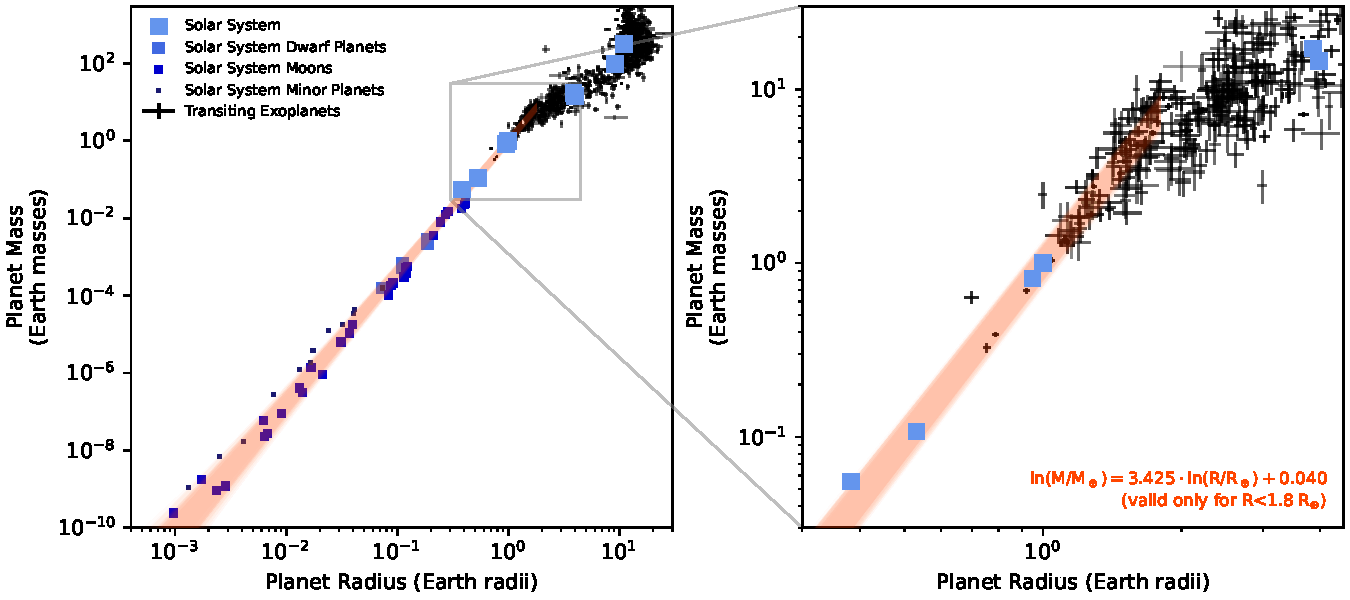
\includegraphics[width=\textwidth]{figures/mass-radius-relation-for-rocky-planets}
\caption{To determine escape velocities for objects without measured masses, we derive an empirical mass-radius relationship from exoplanets (errorbars) and Solar System objects (squares). We use this relation, valid for rocky planets up to $1.8\rm{R}_\earth$, to estimate planet masses and uncertainties that incorporate the intrinsic scatter on the relation, the uncertainties on the model parameters, and uncertainties on the planet radii (\href{https://github.com/zkbt/shoreline/blob/main/notebooks/fit-mass-radius-relation.ipynb}{\texttt{</>}}).
}
\label{f:mass-radius}
\end{figure*}

\subsection{What planets do we label as having atmospheres?}

We define two samples for fitting in \S\ref{s:fitting}, and label planets in each sample as either having an atmosphere ($A_i = 1$) or not  ($A_i = 0$). In both cases, to simplify the analysis, we exclude planets with quoted ages younger than 500 Myr, to minimize having to imagine the future states of still rapidly evolving planets \citep{lopezUnderstandingMassRadiusRelation2014a, chenEvolutionaryAnalysisGaseous2016b,  thaoFeatherweightGiantUnraveling2024b}. 

For our {\bf any atmosphere} sample, we are generous in what we call ``having an atmosphere" ($A_i = 1$), as in ZC17. For Solar System bodies, we include all major planets (everything except Mercury) and moons (Titan) with atmospheric surface pressures $>10^{-6}$ bar. We include outer Solar System moons or dwarf planets that have managed to retain significant volatile reservoirs \citep{schallerVolatileLossRetention2007}, either as seasonally sublimating atmospheres and/or substantial global N$_2$ and CH$_4$ volatile deposits on their surfaces: Triton, Pluto, Makemake, Eris \citep{youngStructureCompositionPlutos2018, sicardyConstraintsEvolutionTriton2024, grundyModerateRatiosMethane2024}. We label all other Solar System objects as $A_i = 0$.

For exoplanets, planets larger than $2.0 \rm {R_\earth}$ are difficult to explain with pure rocky compositions \citep{rogersMost16Earthradius2015b, zengNewPerspectivesExoplanet2021, rogersMostSuperEarthsHave2025}, so we label all planets 
with radii more than 1$\sigma$ over this limit as requiring atmospheres (or significant icy volatiles) to explain their low densities $A_i = 1$. Many planets smaller than $2.0 \rm {R_\earth}$ have atmospheres too, but we apply labels only to those with direct atmosphere measurements, as follows.

We apply $A_i = 1$ to one rocky planet with evidence for atmospheres. 55 Cnc e shows variable JWST eclipse spectra suggesting a (potentially stochastically outgassed) CO/CO$_2$ atmosphere \citep{huSecondaryAtmosphereRocky2024, patelSecondaryAtmosphereRocky2024}. 

We apply $A_i = 0$ to these rocky planets with eclipse observations of hot daysides that strongly suggest low albedos and poor global heat recirculation inconsistent with thick atmospheres \citep[see][]{kollIdentifyingCandidateAtmospheres2019c, mansfieldIdentifyingAtmospheresRocky2019b}. LHS 3844b, Gl 367b, TOI-1685b have a deep eclipses, symmetric phase curves, and dark night sides \citep{kreidbergAbsenceThickAtmosphere2019a, zhangGJ367bDark2024, luqueDarkBareRock2024}. GJ 1252b, TOI-1468b, LHS 1140c have deep photometric eclipses \citep{crossfieldGJ1252bHot2022, meiervaldesHotRocksSurvey2025, fortuneHotRocksSurvey2025a}, and
Gl 486b and GJ 1132b have deep MIRI/LRS spectroscopic eclipses \citep{weinermansfieldNoThickAtmosphere2024, xueJWSTThermalEmission2024a}. 

We leave the following planets unlabeled ($A_i = ?$), meaning the are ignored from the probabilistic fit, even if there have been suggestions they lack atmospheres. 
Kepler-10b and Kepler-78b have symmetric phase curves from Kepler, but with only the optical bandpass their deep eclipses are degenerate between reflected and thermal light, thus complicating atmospheric inferences \citep{sanchis-ojedaTransitsOccultationsEarthsized2013, estevesChangingPhasesAlien2015a, huSemianalyticalModelVisiblewavelength2015, singhProbingKeplersHottest2022}. K2-141 shows a K2 + Spitzer phase curve suggesting a high albedo or hot inversion layer, but whether an atmosphere is absolutely required remains ambiguous \citep{singhProbingKeplersHottest2022, ziebaK2SpitzerPhase2022}. LHS 1478b and TOI-431b appear to have a shallow thermal eclipses, but more data are needed to rule out systematics \citep{augustHotRocksSurvey2025, monaghanLow45Mm2025a}. TRAPPIST-1b and TRAPPIST-1c show deep MIRI eclipses implying hot day sides \citep{greeneThermalEmissionEarthsized2023, ihConstrainingThicknessTRAPPIST12023, ziebaNoThickCarbon2023, ducrotCombinedAnalysis1282025} and no obvious planetary transmission spectrum features \citep{limAtmosphericReconnaissanceTRAPPIST12023, radicaPromisePerilStellar2025, rathckeStellarContaminationCorrection2025}, but systemic stellar uncertainties leave the system still slightly ambiguous \citep{howardCharacterizingNearinfraredSpectra2023, rackhamRobustCorrectionsStellar2024,  fauchezStellarModelsAlso2025}. LTT 1445A b has a deep MIRI/LRS eclipse implying a hot dayside \citep{wachiraphanThermalEmissionSpectrum2025a}, but with the promise that it and LTT 1445A c \citep{passHSTWFC3Light2023} will soon be observed at 15 $\mu$m in the Rocky Worlds program\footnote{\href{https://rockyworlds.stsci.edu/rw-website-targets.html}{rockyworlds.stsci.edu/rw-website-targets.html}} we leave it ambiguous for now. Transmission spectra have not yet conclusively identified nor ruled out the rocky planet atmospheres due to degeneracies with clouds \citep{lustig-yaegerMirageCosmicShoreline2019} and/or stellar contamination \citep{mayDoubleTroubleTwo2023, moranHighTideRiptide2023}; we leave transmission spectroscopy-based non-detections as $A_i = ?$.

%% rocky worlds
%GJ 3929
%LHS 1140b\citep{cadieuxTransmissionSpectroscopyHabitable2024}}
%LTT 1445Ab 
%LTT 1445Ac
%
%% other planets of interest
%TOI 270
%GJ 1214b
%K2-18b
%TOI 3884b 
%TOI 700? 
%Gl 436? 
%GJ 3470? 
%
%% questionable 
%LHS 1478
%TOI 431? 

%L 98-59 may shows hints of an SO2 atmosphere \citep{bello-arufeEvidenceVolcanicAtmosphere2025b}, but the transmission spectrum is also consistent with a flat line so we leave it unlabeled, 


For our {\bf warm CO$_2$ atmosphere} sample, we restrict the above sample to planets with zero-albedo equilibrium temperatures cool enough to have a solid surface \citep[$< 1700\mathrm{K}$;][]{boukareDeepTwophaseHemispherical2022}, trying to avoid magma oceans that might tilt a cosmic shoreline by providing direct contact with a much deeper volatile reservoir \citep[see][]{huSecondaryAtmosphereRocky2024}. We also limit to temperatures warm enough for CO$_2$ to be gaseous ($>$194 K, where the saturation vapor pressure for CO$_2$ is 1 bar; \citealt{pierrehumbertPrinciplesPlanetaryClimate2010}), coinciding approximately with the outer edge of the habitable zone \citep[where CO$_2$ can no longer provide greenhouse warming because it condenses out of the atmosphere;][]{kopparapuHabitableZonesMainsequence2013}. We focus on CO$_2$ and O$_2$ (which condenses at even colder temperatures) as likely major constituents of temperate atmospheres, especially those that have been distilled by near-complete atmospheric erosion \citep{hamanoEmergenceTwoTypes2013a, lugerExtremeWaterLoss2015, schaeferPredictionsAtmosphericComposition2016c,  krissansen-tottonErosionLargePrimary2024}. Venus (92 bar) and Mars ($0.004-0.009$ bar) are both about 95\% CO$_2$ \citep{loddersPlanetaryScientistsCompanion1998}, and Earth too would likely have about 100 bars of atmospheric CO$_2$ (swamping our 1 bar of N$_2$ + O$_2$; \citealt{ingersollPlanetaryClimates2013}) if not for the presence of H$_2$O continually raining down, dissolving atmospheric CO$_2$, and locking it away into solid carbonates \citep{walkerNegativeFeedbackMechanism1981, lecuyerComparisonCarbonNitrogen2000, wordsworthAtmospheresRockyExoplanets2022, hansenDetectingAtmosphericCO22025}. Earth preserves its H$_2$O (and thus keeps our CO$_2$ trapped in limestone deposits) only because water precipitates before it reaches the upper atmosphere, where it would be dissociated by UV radiation and its H atoms lost to space. On warm Venus, the runaway greenhouse process \citep{komabayasi1ChengFen2XiangXinoDaQiQuantoShuiQuanwoYousuruJiaXiangDenaHuoXinggaYiDingnoTaiYangGuangXiadetoriuruBuLianSoknaPingHengWenDunituite1ChengFen2XiangXinoDaQiQuantoShuiQuanwoYousuruJiaXiangDenaHuoXinggaYiDingnoTaiYangGuangXiadetoriuruBuLianSoknaPingHengWenDunituiteDiscreteEquilibriumTemperatures1967, ingersollRunawayGreenhouseHistory1969} vaporizes water and drives it inevitably to the upper atmosphere, where its H escapes \citep{hamanoEmergenceTwoTypes2013a, leconteIncreasedInsolationThreshold2013, wordsworthWaterLossTerrestrial2013}. On cold Mars, hydrogen has also been preferentially lost \citep{jakoskyLossMartianAtmosphere2018}, with modern escape largely driven by dust dynamics carrying frozen water up to high altitudes \citep{chaffinMartianWaterLoss2021}. CO$_2$ (possibly mixed with O$_2$) atmospheres are also particular detectable for exoplanets with JWST, especially with Rocky Worlds' use of MIRI filter photometry centered on the strong 15 $\mu$m CO$_2$ absorption band \citep{morleyObservingAtmospheresKnown2017b, ihConstrainingThicknessTRAPPIST12023}. 

By comparing the broader {\bf any} sample to the smaller zoomed-in {\bf warm CO$_2$} sample, we can test whether we see evidence for the shoreline changing from the global scale (all planets, all volatiles) to the local scale (temperate rocky planets). In both cases, we caution that for exoplanets the direct observational constraints on the absence of atmospheres ($A_i = 0$) does {\em not} mean planets necessarily have no atmosphere at all; for tidally locked planets, a JWST measurement of hot dayside emission might only constrain the atmospheric pressure on an individual planet to less than about 10 bar \citep{kollScalingAtmosphericHeat2022}, really saying simply that we have not detected a very thick Venus-like atmosphere.

%Although Earth's 2025 atmosphere is 430 ppm $\rm{CO_2}$, we include it as a thick $\rm{CO_2}$ atmosphere because 


\section{Fitting a Cosmic Shoreline}
\label{s:fitting} 

We construct a generative model that tries to explain the atmosphere labels $A_i$ for planet $i$ using the predictors $f_i$, $v_{\sf esc, i}$, $L_{\star, i}$. We first define a cosmic shoreline flux $f_{\sf shoreline}$ with the power law expression

\begin{equation}
f_{\sf shoreline} = f_{\sf 0} \left(\frac{v_{\sf esc}}{v_{\sf esc, \oplus}}\right)^p\left(\frac{L_\star}{L_\odot}\right)^q
\end{equation}
where $f$ is also in units relative to Earth, with $f = 1$ corresponding to $f = f_\earth = 1360 \mathrm{W/m^2}$. This power law log transforms to a linear plane
\begin{equation}
\label{e:log_f_shoreline}
 \log_{10} f_{\sf shoreline}  =  \log_{10} f_{\sf 0} + p \cdot  \log_{10} \left(\frac{v_{\sf esc}}{v_{\sf esc, \oplus}}\right) + q \cdot  \log_{10} \left(\frac{L_\star}{L_\odot}\right)
\end{equation}
for parameters $f_{\sf 0}$, $p$, $q$. We define a distance from this shoreline in log-flux as 
\begin{equation}
\label{e:delta}
\Delta =  \log_{10} f - \log_{10}f_{\sf shoreline}
\end{equation}
which is similar to the Atmosphere Retention Metric from \citet{passRecedingCosmicShoreline2025}. We use this distance to describe the probability of each planet having an atmosphere with the logistic function
\begin{equation}
p_i = P(A_i = 1 | \mathbf{x}_i, \boldsymbol{\theta} ) = \frac{1}{1+e^{\Delta_i/w}}
\label{e:p_i}
\end{equation}
where $\mathbf{x}_i = [\log_{10}(f_i/f_\earth), \log_{10} (v_{esc, i}/v_{esc, \earth}), \log_{10} (L_{\star, i}/L_\sun)]$ are the predictors for each datum and $\boldsymbol{\theta} = [f_{\sf 0}, p, q, w]$ are the model parameters. This logistic function smoothly transitions from 1 when $f$ is below the shoreline to 0 above, with the width parameter $w$ describing how quickly in $\log_{10} f$ planets change from mostly having atmospheres to mostly not. The likelihood of the data ensemble $\mathbf{A}$ can be calculated by multiplying $p_i^{A_i}$ (= how well did we predict the presence of an atmosphere) by $(1-p_i)^{1-A_i}$ (= how well did we predict the absence of an atmosphere) across all data points:

\begin{equation}
P(\mathbf{A} | \boldsymbol{\theta}) = \prod_{i=1}^{N} p_i^{A_i} \cdot (1-p_i)^{1-A_i}
\end{equation} 
This likelihood $P(\mathbf{A} | \boldsymbol{\theta})$
 together with a prior $P(\boldsymbol{\theta})$ determine the posterior probability $P(\boldsymbol{\theta} | \mathbf{A}) = P(\mathbf{A} | \boldsymbol{\theta}) P(\boldsymbol{\theta})$. For $f_{\sf 0}$, we adopt an uninformative uniform prior on $\log_{10} f_{\sf 0}$. For $p$, and $q$, we adopt the uninformative prior $P(\boldsymbol{\theta}) \propto (1+p^2)^{-3/2}\cdot (1+q^2)^{-3/2}$, which avoids the infinitely growing prior space toward high slope values and effectively represents a uniform prior on the rotation angle of the slopes in log space \citep[see][]{vanderplasFrequentismBayesianismPythondriven2014a}. For $w$, we adopt a uniform prior of $-4 > \ln w > 2$,  spanning $0.018~\mathrm{dex} < w < 7.4~\mathrm{dex}$, or from a 4.3\% change in $f$ at the narrowest to a factor of $2.5\times10^7$ change in $f$ at the widest; practically we find that allowing narrower widths than this can reveal sharp discontinuities that become difficult to sample. 

To account for measurement uncertainties on the predictors, the expression for $p_i$ in Equation \ref{e:p_i} should be marginalized over the distribution of true (unknown) values for each planet's $\mathbf{x}_i$. While this marginalization can sometimes be done analytically (as in the mass-radius fit in \S\ref{f:mass-radius}), we were unable to find a simple analytic expression and instead relied on the {\em remarkable} efficiency of \texttt{numpyro}'s NUTS sampler to do this marginalization numerically. We introduced three parameters for {\em each} datapoint (933 planets for {\bf any}, 496 planets for {\bf warm CO$_2$}) to represent the true values of $\mathbf{x}_i$ with normal priors centered on the measured values and the uncertainties as their widths, and we sampled these alongside the 4 parameters $\boldsymbol{\theta}$. 

We used \texttt{numpyro} with NUTS to sample from this posterior, running 4 chains with 5,000 warm-up steps and 50,000 samples each, always achieving a Gelman-Rubin statistic of 1.0 across the chains and usually achieving an effective sample size always (and sometimes much) larger than 1,000. Even with the thousands of hyperparameters we use to marginalize over measurement uncertainties, this samping takes only a few minutes on a modern MacBook Pro. 







\section{Shorelines in 3D}
\label{s:shorelines}

We start by discussing the qualitative behavior of the inferred shorelines, reserving more quantitative discussion of parameter values and uncertainties for \S\ref{s:slopes}. Figure \ref{f:shoreline-any} shows the inferred shoreline model for the {\bf any} atmosphere subset, representing the question of whether a planet has any type of atmosphere or volatile reservoir across a broad range of flux, similar to ZC17. Because the probability of an atmosphere $A$ is a function in a 3D volume defined by $f$, $v_{\sf esc}$, $L_\star$, it can be a little tricky to visualize. We display this 3D volume with slices, each row holding one dimension fixed to a narrower range and visualizing the other two dimensions on the $x$ and $y$ axes, and each column displaying a different range of values for the fixed dimension. The background color shows the modeled probability of an atmosphere at each $(x, y)$ location in each slice, marginalized (= integrated, see \citealt{hoggDataAnalysisRecipes2010a, siviaDataAnalysisBayesian2011, vanderplasFrequentismBayesianismPythondriven2014a, ivezicStatisticsDataMining2020}) over both the width of the slice and the uncertainties on the model parameters. Even for infinitely thin slices with no parameter uncertainties the transition would still appear fuzzy due to the intrinsic width $w$ (see Equation \ref{e:p_i}). 

\begin{figure*}[ht!]
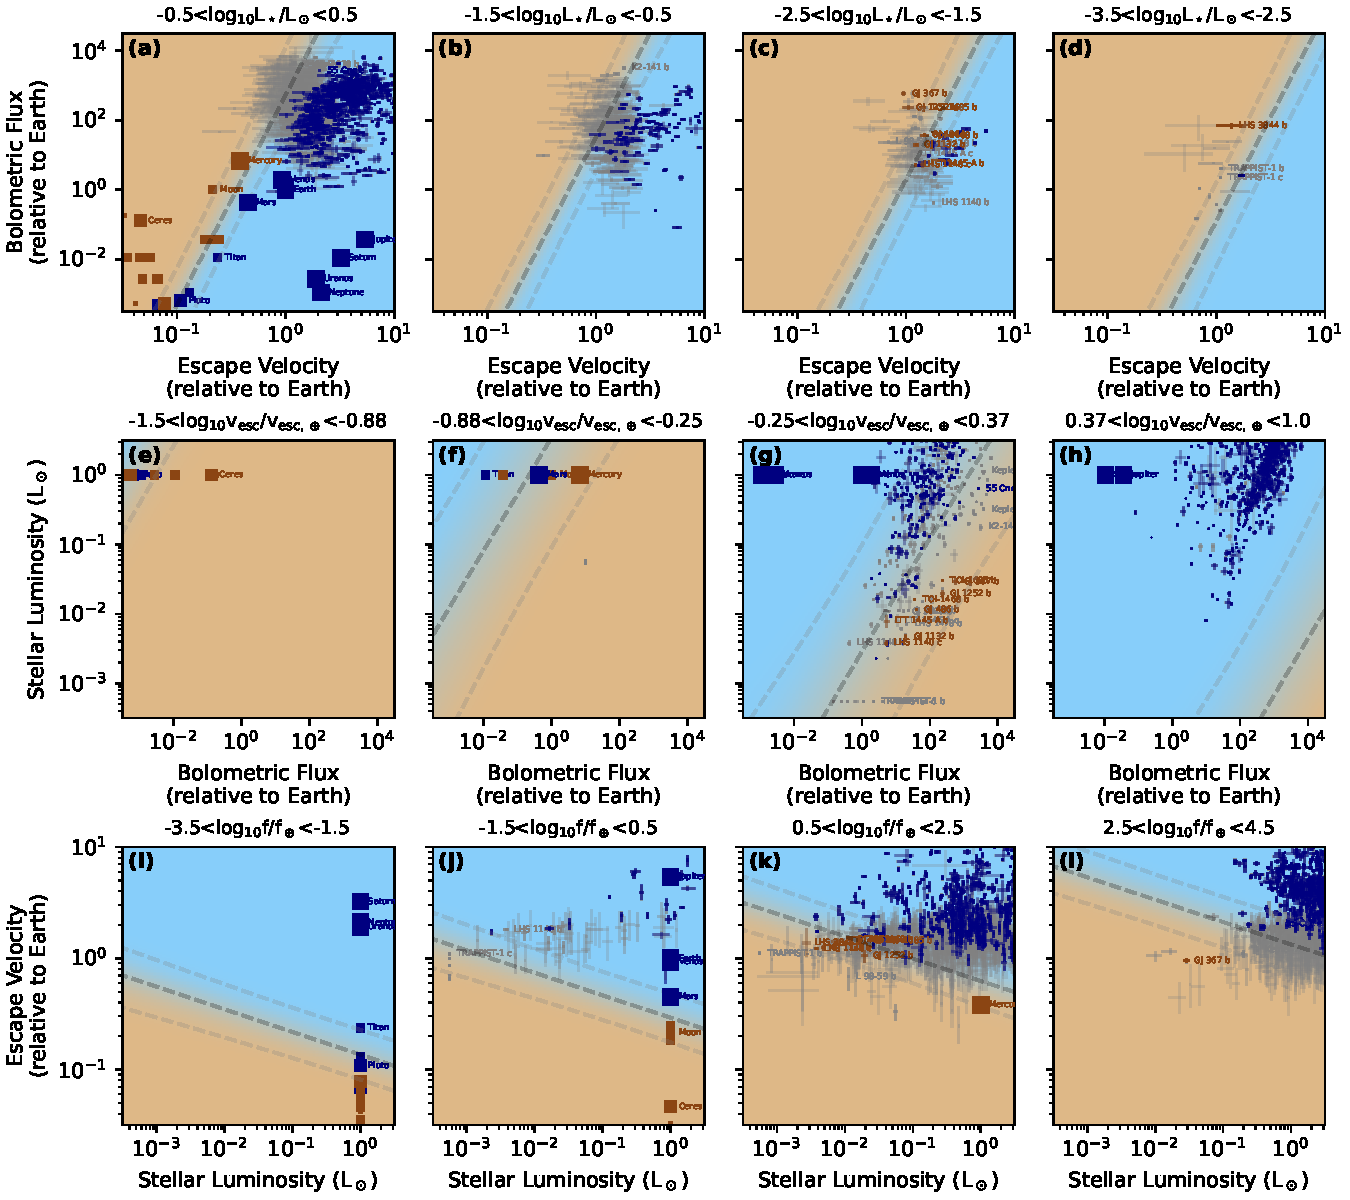
\includegraphics[width=\textwidth]{figures/grid-of-shorelines-any.pdf}
\caption{A cosmic shoreline dividing exoplanets (errorbars) and Solar System planets (squares) with any type of atmosphere or global surface volatiles (blue symbols) from those without (brown symbols). The shoreline defines a plane in the 3D space of ($f$, $v_{\sf esc}$, $L$); each row shows slices that consider a narrow range of stellar luminosity (top), planet escape velocity (middle), and planet flux (bottom). Background colors indicate the modeled probability of an atmosphere at each location (sandy brown for $p_i = 0$, water blue for $p_i$ = 1), accounting for the intrinsic width of the shoreline and marginalizing over the parameter uncertainties and the width of the slice. For context, the shoreline most relevant to an Earth-like planet ($L_\star = 1L_\sun$ for top row, $v_{\sf esc} = v_{\sf esc, \earth}$ for middle row, $f = f_\earth$ for bottom row) is repeated across slices (dotted lines \todo{NEED TO ADD!).}}
\label{f:shoreline-any}
\end{figure*}


The top row (a-d) of Figure \ref{f:shoreline-any} holds $L_\star$ as the fixed dimension, decreasing from solar type host stars on the left and moving toward the latest possible M dwarf stars on the right. The centers of these luminosity ranges (1$L_\sun$, 0.1$L_\sun$, 0.01$L_\sun$, 0.001$L_\sun$) correspond to main-sequence spectral types (G2, K7, M3.5, and M6) according to the \citet{pecautINTRINSICCOLORSTEMPERATURES2013} sequence. The upper left panel shows $v_{\sf esc}$ and bolometric flux $f$ for both Solar System objects (all with $L = 1.0L_\sun$) and exoplanets with host stars within a factor of $\sqrt{10}$ of the Sun's luminosity; it is the closest analog to Figure 1 from ZC17, which shows similar quantities but without the restriction on exoplanet host star type. The shoreline in this row has a slope of $p$ (see Equation \ref{e:log_f_shoreline}) and reading from left to right appears to recede \citep[to borrow a visual metaphor from][]{passRecedingCosmicShoreline2025} down and to the right, with the bolometric threshold $f_{\sf shoreline}$ decreasing at fixed $v_{\sf esc}$ toward lower luminosity stars. 

The middle row (e-h) shows shoreline slices for different fixed $v_{\sf esc}$, increasing from tiny low-mass dwarf planets on the left to gas giants on the right. Only Solar System objects are known at low $v_{\sf esc}$ (e), but for Earth-like $v_{\sf esc}$ (g) exoplanet atmosphere data are available either as radii large enough to require volatiles or as rocky planets with JWST hot dayside brightness temperatures disfavoring thick atmospheres. These constraints trace out the slope $1/q$, showing that cooler less luminous stars also have lower maximum allowable flux levels $f_{\sf shoreline}$ for atmospheres to survive. 

The bottom row (i-l) shows the shoreline for different fixed $f$, increasing from the cold outer regions of the Solar System on the left to the very hottest exoplanets on the right. The slope of the shoreline in this projection is $-q/p$ and indicates a larger $v_{\sf esc}$ is necessary in order for lower $L_\star$ hosts to permit atmospheres. For temperate planets (j), if we imagine shrinking the host star luminosity while keeping $f$ constant, Mars-sized planets would be unable to retain atmospheres around stars less luminous than $0.1 L_\sun$, and Earth/Venus-size planets would likely lose atmospheres somewhere between $10^{-3} - 10^{-2} L_\sun$.

Figure \ref{f:shoreline-CO2} shows the shoreline inferred for the zoomed-in {\bf warm CO$_2$} sample of planets, including only those with equilibrium temperatures warm enough for CO$_2$ to remain in gaseous form and cool enough to not necessitate a dayside magma ocean. Focusing on the local geography of the cosmic shoreline more relevant to JWST, the most important differences are (a) the absence of the ultrahot atmospheres 55 Cnc e and K2-141 at high $f$ and (b) the lack of small icy objects to anchor the slope down at low $f$. We see the same qualitative story as before: less luminous stars create harsher environments for planetary atmospheres. 

\begin{figure*}[ht!]
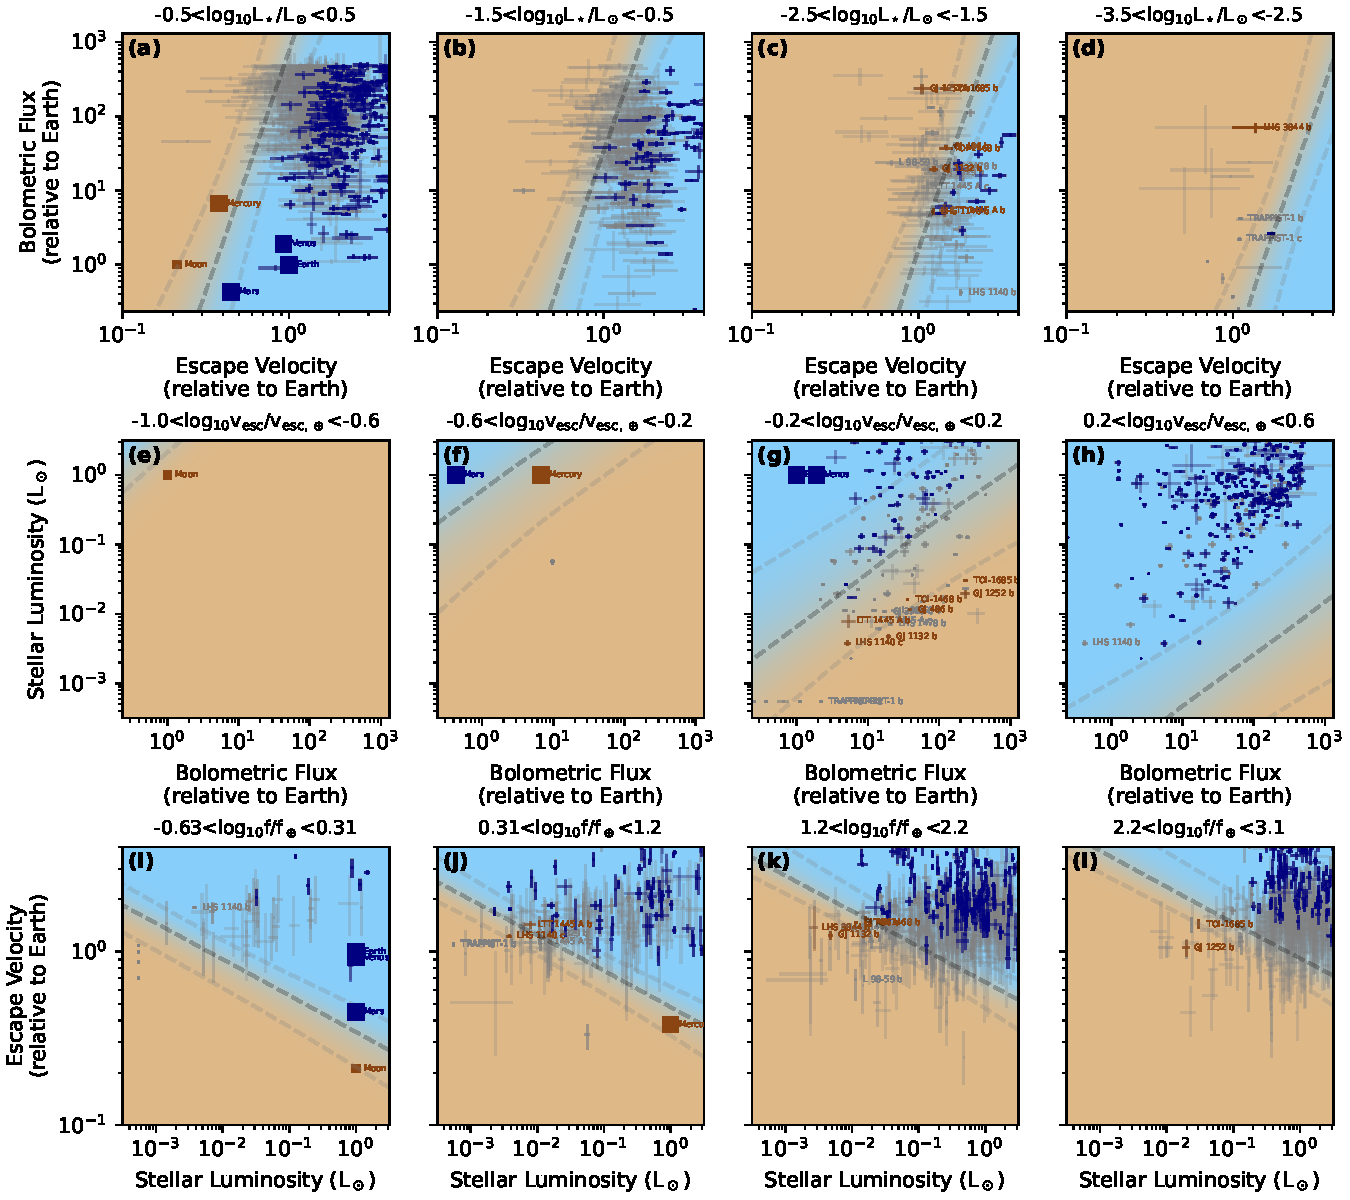
\includegraphics[width=\textwidth]{figures/grid-of-shorelines-CO2.pdf}
\caption{A cosmic shoreline exactly as in Figure \ref{f:shoreline-any}, but specifically targeting $\rm{CO}_2$-dominated atmospheres on planets with equilibrium temperatures warm enough $\rm{CO_2}$ to exist as a gas (a sublimation temperature of ${\rm T_{CO_2}}= ??? \mathrm{K}$) and cool enough that a global magma ocean is less likely (${\rm T_{magma}} = ?? \mathrm{K}$ from ???). This more narrowly defined cosmic shoreline matters because $\rm CO_2$ is both likely in warm secondary atmospheres and relatively easier to detect for exoplanets in thermal emission with JWST.}
\label{f:shoreline-CO2}
\end{figure*}

\begin{figure*}[ht!]
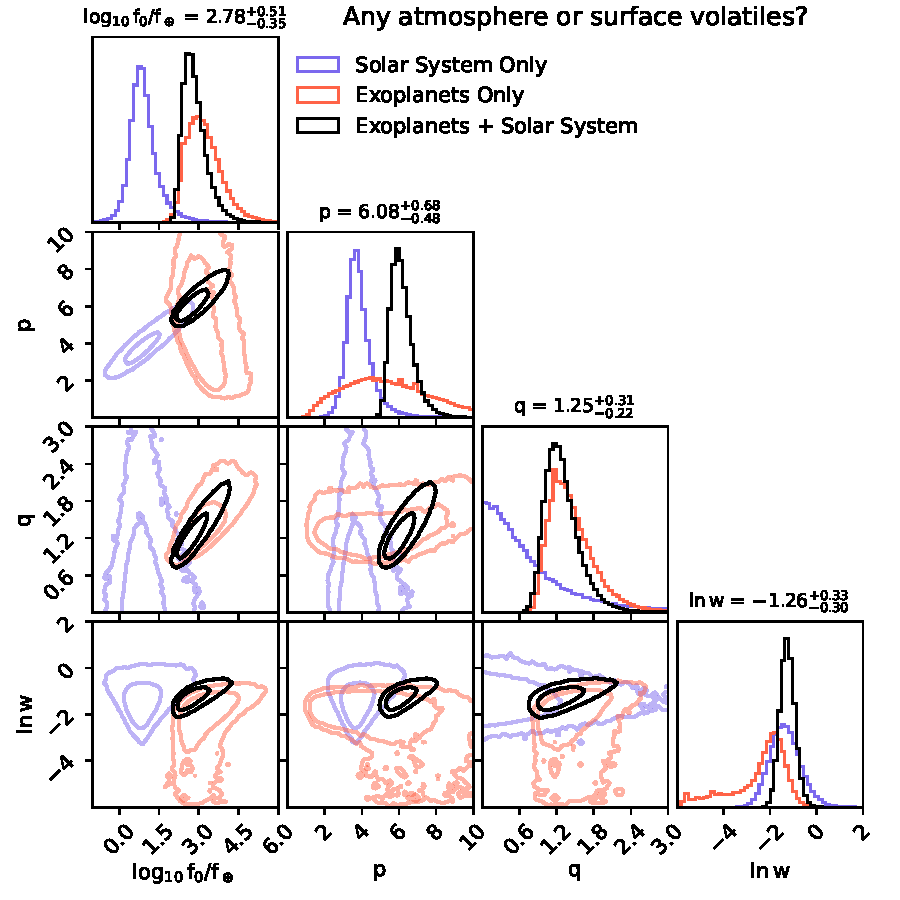
\includegraphics[width=\textwidth]{figures/posteriors-any.pdf}

\caption{Cosmic shoreline parameter posterior probabilities for {\bf any} atmosphere or surface volatiles, corresponding to data in Figure \ref{f:shoreline-any}. Panels show marginalized 1D histograms (diagonal) and marginalized 2D distributions (off-diagonal) with contours that enclose 68.3\% and 95.4\% probability. Titles along the diagonal show confidence intervals for the exoplanets + Solar System joint fit. The model parameters define a shoreline via $\log_{10} f_{\rm shoreline} = \log_{10} f_{0} + p \log_{10} (v_{\sf esc}/v_{\sf esc, \earth}) + q \log_{10} (L_\star/L_\sun)$, with $w$ representing the logistic width parameter setting the fuzziness of the shoreline.}
\label{f:posteriors-any}
\end{figure*}


\begin{figure*}[ht!]
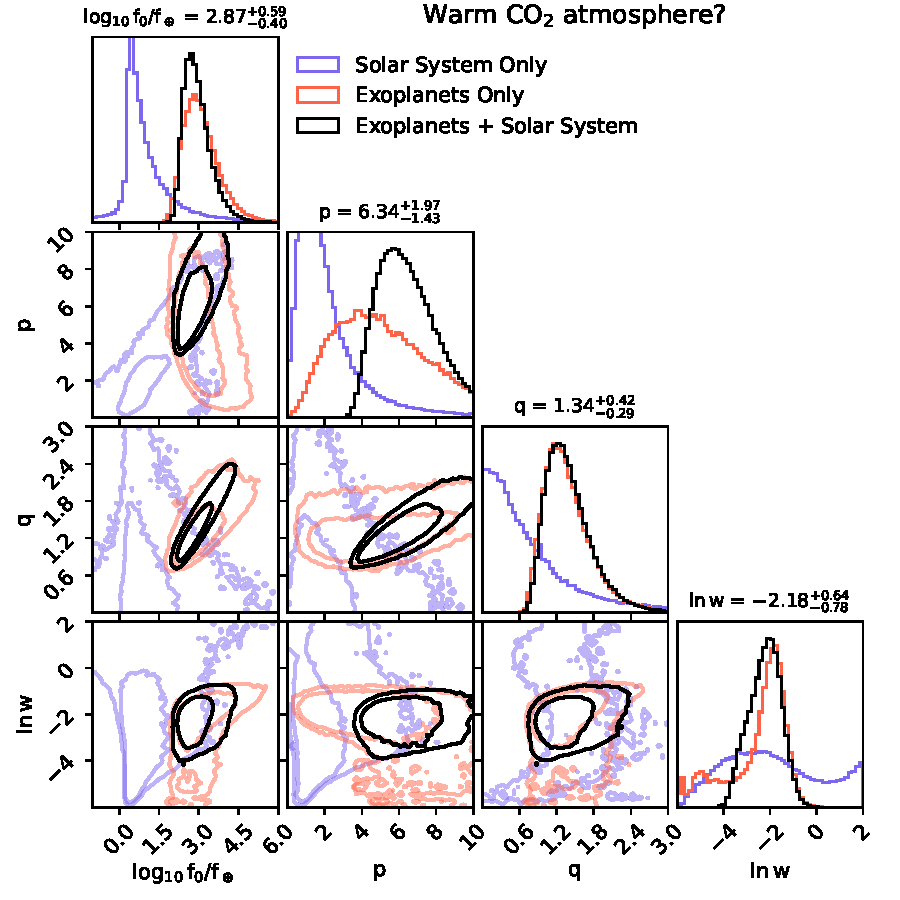
\includegraphics[width=\textwidth]{figures/posteriors-CO2.pdf}

\caption{Cosmic shoreline parameter posterior probabilities for {\bf warm CO$_2$} atmosphere or surface volatiles, corresponding to data in Figure \ref{f:shoreline-CO2}. Panels show marginalized 1D histograms (diagonal) and marginalized 2D distributions (off-diagonal) with contours that enclose 68.3\% and 95.4\% probability. Titles along the diagonal show confidence intervals for the exoplanets + Solar System joint fit. The model parameters define a shoreline via $\log_{10} f_{\rm shoreline} = \log_{10} f_{0} + p \log_{10} (v_{\sf esc}/v_{\sf esc, \earth}) + q \log_{10} (L_\star/L_\sun)$, with $w$ representing the logistic width parameter setting the fuzziness of the shoreline.}
\label{f:posteriors-CO2}
\end{figure*}

\begin{figure*}[ht!]
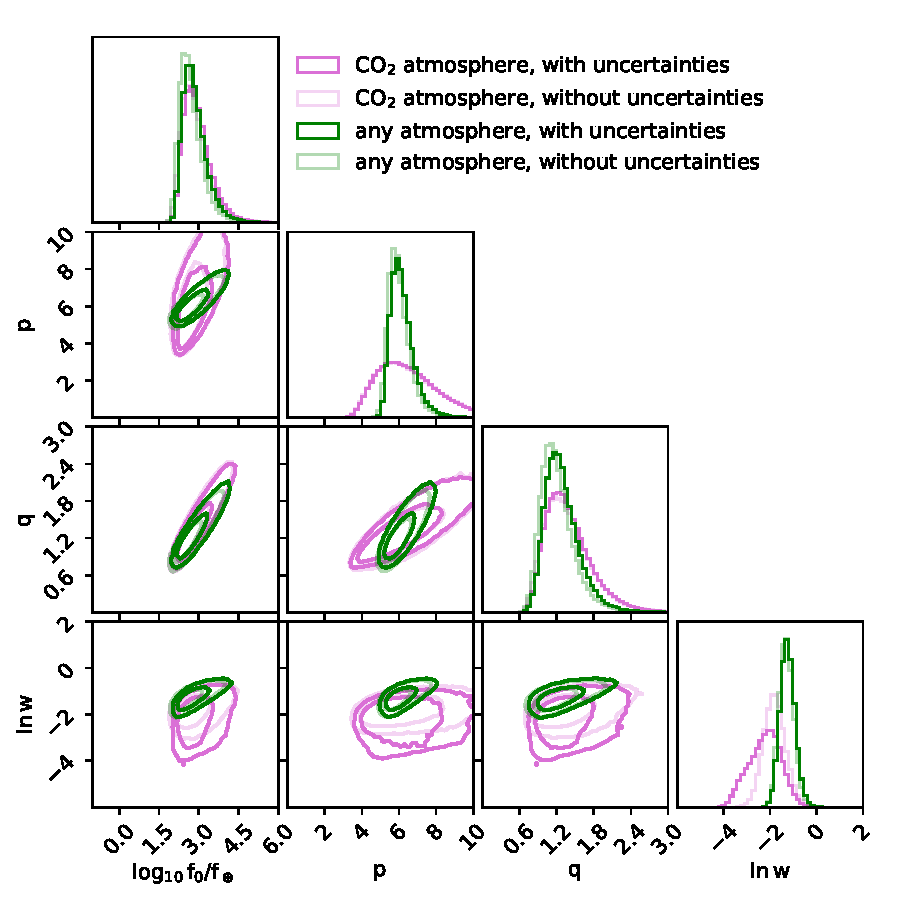
\includegraphics[width=\textwidth]{figures/posteriors-with-and-without-uncertainties.pdf}

\caption{Posteriors inferred with (intense lines) and without (faint lines) accounting for uncertainties on planet properties ($f$, $v_{\sf esc}$, $L_\star$). Both types of atmosphere are shown, using exoplanet and Solar System data in all fits. Marginalizing over uncertainties broadens the possible intrinsic shoreline widths $w$ to lower values but does not significantly shift the other parameters setting the shoreline shape.}
\label{f:posteriors-uncertainties}
\end{figure*}


\section{Interpeting the Shoreline Parameters}
\label{s:slopes}

Figures \ref{f:posteriors-any} and  \ref{f:posteriors-CO2} show posterior probability distributions for our shoreline parameters. In addition to the joint fits, which include all planets together, we also show posteriors for what we might learn from just Solar System or just exoplanets each by themselves. We compare these posteriors with \texttt{corner.py} \citep{foreman-mackeyCornerpyScatterplotMatrices2016}, with contours in each 2D panel that enclose 68.3\% and 95.4\% of the probability marginalized over other parameters. 


\subsection{The shoreline for {\bf any} atmosphere}
From the joint fit considering any kind of atmosphere or surface volatiles (Figure \ref{f:posteriors-any}), we find the intercept to be $\log_{10}{f_0} = 2.82_{-0.34}^{+0.49}$, meaning that an Earth-size planet orbiting a Sun-like star should on average be able to retain an atmosphere with $f/f_\earth$ up to about $10^{2.81} = 650$. If we moved Earth inward toward the Sun, hydrogen and the hope of habitability would be lost long before this limit, likely leaving heavily oxidized CO$_2$/O$_2$ atmospheres.

The escape velocity slope $p = 6.16_{-0.47}^{+0.65}$ is marginally steeper than $p=4$ chosen by ZC17 and means that a factor of $10\times$ increase in $v_{\sf esc}$ causes the critical flux $f_{\sf shoreline}$ to move up by $10^{6.16}$. Notably, for Solar System planets alone we find $p = 3.76_{-0.51}^{+0.72}$ and for exoplanets alone we find $p = 6.6 \pm 2.8$ (both consistent with $p=4$), so the higher consensus joint slope reflects a particular compromise where these two different samples that mostly occupy different regions of parameter space can agree.

The stellar luminosity slope $q = 1.21_{-0.23}^{+0.30}$ means that if we decrease the luminosity of the host star by $10\times$, the maximum flux that permits atmospheres $f_{\sf shoreline}$ decreases by a factor $10^{1.21}$. This is steep! If we take $f_{\sf hz} = f_\earth = 1360 \mathrm{W/m^2}$ as a crude approximation for the habitable zone (neglecting the important dependence on the stellar spectrum; \citealt{kopparapuHabitableZonesMainsequence2013}), this fit implies $f_{\sf shoreline} < f_{\sf hz}$ for stars less luminous than ?? (roughly M? spectral type, ? mass, ? radius, ? teff). Cast in terms of semimajor axis $a$, the habitable zone distance necessarily shrinks toward smaller stars as $a_{\sf hz} \propto L_\star^{1/2}$ \citep[generally making them easier to observe;][]{blakeNearInfraredMonitoringUltracool2008, nutzmanDesignConsiderationsGroundBased2008a}. The shoreline distance scales as $a_{\sf shoreline} \propto L_\star^{(1-q)/2}$, so $q > 1$ means that $a_{\sf shoreline}$ grows larger toward smaller stars, with ominous prospects for atmospheric retention around the coolest stars.

The intrinsic width of the shoreline $\ln w = -1.185 \pm 0.298$, or $w = 0.31\pm??~\mathrm{dex}$, means than if $f$ increases by a factor of $10^{0.31} = 2.0$ above $f_{\sf shoreline}$ then the probability of an atmosphere drops from $50\%$ to $1/(1 + e^{1}) = 27\%$ (Equation \ref{e:p_i}). To translate into more familiar 1$\sigma$ and 2$\sigma$ probabilities from a normal distribution, the chance of having an atmosphere drops to 16\% and 5\% at $1.7w$ and $2.9w$, respectively. The transition from 95\% to 5\% probability of having an atmosphere spans a factor of $10^{5.8w}$ in flux, or $63\times$, seen as the blending of colors in Figure \ref{f:shoreline-any}. 


%For a star like TRAPPIST-1 at $\log_{10} (L_\star/L_\sun) = -3.26 \pm 0.01$ \citep{ducrotTRAPPIST1GlobalResults2020}, a value of $q=1.21$ implies the shoreline for an Earth-mass planet ($v_{\sf esc} = v_{\sf esc, \earth}$) occurs at $f_{shoreline} = 0.075 f_\earth$ or $a_{\sf shoreline} = 

\subsection{The shoreline for {\bf warm CO$_2$} atmospheres}

From the joint fit focusing only on temperate rocky planets and their likely CO$_2$-rich compositions (Figure \ref{f:posteriors-CO2}), we find $log_{10} f_0 = 2.42_{-0.28}^{+0.43}$, $p = 5.19_{-0.99}^{+1.5}$, and $q = 0.979_{-0.18}^{+0.3}$ for the shape of the shoreline. 
Figure \ref{f:posteriors-uncertainties} shows the joint fits for both samples, permitting more direct comparison between the two. Relative to the any atmosphere fits, the CO$_2$ parameter uncertainties are larger, probably due to the narrower range of fluxes providing leverage on the slope. Slopes nudge toward marginally shallower, but not significantly so. 

The biggest difference is $\ln w = -2.91 \pm 0.73$ being much lower for the narrower, with a transition from 95\% to 5\% atmosphere probability spanning 0.65 dex or a factor of $4.5\times$. One possibility is that the width $w$ on broad global scales is partially capturing unknown curvature or topography along the shoreline, and a lower $w$ in the zoomed-in sample might hint at the log-linear shoreline being a better local description on increasingly fine scales. Testing this hypothesis will require many more planets with reliable atmosphere labels. 

% SHOULD I REARRANGE TO any THEN CO2
\subsection{Sensitivity to Including Gas Giant Planets}
In both these fits, we did not place upper limits on planet escape velocity or radius, allowing all giant planets to participate in sculpting the shoreline, as in ZC17. Hot Jupiters could potentially bias the shoreline slope, in that they might have lost tens of Earth masses of atmosphere but still appear to meet our atmosphere criteria. We tested the sensitivity of the inferred shoreline to this concern by repeating the fits with but including only planets smaller than Neptune; we found no significant changes to the parameter posteriors. 

\subsection{Sensitivity to Planet Parameter Uncertainties}
We test the impact that measurement uncertainties on the predictors $v_{esc}, f, L_\star$ have the inferred shoreline. Figure \ref{f:posteriors-uncertainties} shows parameter posteriors with and without including parameter uncertainties. Including them slightly broadens distributions and can allow for lower values of $w$, where disagreeing labels at fixed distance from the shoreline can be a little more explained by uncertainties on the predictors and a little less with the intrinsic fuzziness. Still, the differences are surprisingly minor. We hypothesize this is because most parameter uncertainties are smaller than the effect of the intrinsic width $w$. 

\subsection{Physical Interpretation}
Atmospheric loss is fundamentally a matter of energy balance: whatever energy a planet receives from its star (or still-cooling interior; see \citealt{guptaSculptingValleyRadius2019}), must either radiate away or be carried away in the gravitational potential energy of escaping gas \citep{lewisPlanetsTheirAtmospheres1984, chamberlainTheoryPlanetaryAtmospheres1987}. The incoming energy need not be radiative, with particles and fields in the stellar wind also driving loss, and moreso during coronal mass ejections \citep{lammerCoronalMassEjection2007, jakoskyMAVENObservationsResponse2015}. Modeling efforts beyond ZC17 have included various atmospheric sources and sinks to understand where atmospheres can or cannot flourish \citep{tianTHERMALESCAPESUPER2009,
lugerHabitableEvaporatedCores2015, 
owenEvaporationValleyKepler2017, 
wyattSusceptibilityPlanetaryAtmospheres2020, 
guptaCaughtActCorepowered2021,
chatterjeeNovelPhysicsEscaping2024, 
chinRolePlanetaryRadius2024a, 
giallucaImplicationsThermalHydrodynamic2024,
teixeiraCarbondeficientEvolutionTRAPPIST1c2024,
zengCosmicHydrogenIce2024,
vanlooverenAiryWorldsBarren2024,
vanlooverenHabitableZoneAtmosphere2025, 
leeCarvingEdgesRocky2025,
jiCosmicShorelineRevisited2025}. Here, we briefly try to contextualize the newly inferred shoreline parameters through the lens of hydrodynamic escape, as the most efficient path for atmospheric erosion in extreme environments where XUV heating can overwhelm infrared cooling in the tenuous upper atmosphere and drive fluid flows \citep{sekiyaDissipationRareGases1980, watsonDynamicsRapidlyEscaping1981}. 

For the flux slope $p$, we can consider a simplified model of energy-limited escape, where some fraction $\epsilon_{\sf esc}$ of incoming power from $f_{\sf XUV}$ radiation converts directly into gravitational potential energy of outflowing atmosphere \citep{watsonDynamicsRapidlyEscaping1981}, can be written as $\epsilon_{\sf esc} f_{\sf XUV} \pi R_{\sf XUV}^2 \approx GM \dot{M}_{\sf atm}/R_{\sf atm}$ with $\pi R_{\sf XUV}^2$ as the planet's cross-section to high-energy radiation, $\dot{M}_{\sf atm}$ is the atmospheric mass loss rate, and $R_{\sf atm}$ is the effective radius from which atmosphere is escaping. If we neglect important radiative and tidal effects \citep[see][]{lammerAtmosphericLossExoplanets2003, erkaevRocheLobeEffects2007}, crudely approximate $R_{\sf XUV} \approx R_{\sf atm} \approx R$, parameterize the high-energy flux as some fraction of the bolometric flux $f_{\sf XUV} = \epsilon_{\sf XUV} f$,  imagine the atmospheric volatile budget eroded over the system age $t$ to be some fraction of planet mass $\dot{M}_{\sf atm} = \epsilon_{\sf atm} M/t$, and define $\epsilon_{\sf ?} = \epsilon_{\sf atm} \cdot \epsilon_{\sf esc}^{-1} \cdot \epsilon_{\sf XUV}^{-1}$ as a wildly uncertain combined efficiency factor, we would find a shoreline that scales with bolometric flux as $f \propto \epsilon_{\sf ?}  M^2/R^3  \propto \epsilon_{\sf ?}  v_{\sf esc}^4/R  \propto \epsilon_{\sf ?}  v_{\sf esc}^3\sqrt{\rho}$ as in Figure 3 of ZC17. If we further use the mass-radius relation in Figure \ref{f:mass-radius} to estimate $R\propto v_{\sf esc}^{0.85}$ or $M \propto v_{\sf esc}^{2.85}$ for rocky planets, this shoreline can be approximated as $f \propto  \epsilon_{\sf ?}  v_{\sf esc}^p$ with $p \approx$. Strong dependencies lurk inside $\epsilon_{\sf ?}$ that could tilt the flux slope $p$ away from this cartoon $p=3.15$ value, either globally or locally: $\epsilon_{\sf atm}$ depends on volatile delivery history, interior-atmosphere exchange, instellation, and tides \citep{elkins-tantonRangesAtmosphericMass2008, schaeferPredictionsAtmosphericComposition2016c, kiteAtmosphereinteriorExchangeHot2016, seligmanPotentialMeltingExtrasolar2024}, and $\epsilon_{\sf esc}$ depends on instellation, planet mass, and composition \citep{murray-clayAtmosphericEscapeHot2009, owenPlanetaryEvaporationUV2012, owenEvaporationValleyKepler2017, chatterjeeNovelPhysicsEscaping2024, jiCosmicShorelineRevisited2025, leeCarvingEdgesRocky2025}.

Another useful reference slope $p$ comes from a common threshold for mass loss: the escape parameter $\lambda = E_{\sf grav}/E_{\sf thermal} = v_{\sf esc}^2/v_{\sf thermal}^2$, where $v_{\sf thermal} = \sqrt{2k_{\sf B} T/m}$  is the thermal speed of the gas, with $k_{\sf B}$ as the Boltzmann constant, $T$ as temperature, and $m$ as the mass each escaping atom/molecule \citep[see][]{schallerVolatileLossRetention2007, johnsonExospheresAtmosphericEscape2008, gronoffAtmosphericEscapeProcesses2020}. If we calculate this escape parameter $\lambda$ with planets' zero-albedo instantaneous equilibrium temperature $T = T_{\sf eq}  \propto f^{1/4}$ (horribly inaccurately for thick atmospheres by ignoring XUV heating, but effectively setting a lower limit on atmospheric temperatures), constant values $\lambda$ would correspond to $v_{\sf esc}^2 \propto f^{1/4}$ and a shoreline slope $p=8$. The slope in energy-limited escape is  shallower than this because XUV-heated exospheres converge through infrared cooling thermostats to similar hot temperatures despite strongly varying incoming fluxes \citep{chamberlainUpperAtmospheresPlanets1962, murray-clayAtmosphericEscapeHot2009, chatterjeeNovelPhysicsEscaping2024}. That our inferred slopes $p=??\pm??$ (any) or $p=??\pm??$ (warm CO$_2$) fall between these limits is encouraging, but gleaning reliable insights into atmospheric evolution may require more detailed predictive modeling of the flux slope $p$. 

For the stellar luminosity slope $q$, we can interpret it as setting the fraction of light a star emits as XUV via $\epsilon_{\sf XUV} = L_{\sf XUV}/L_{\star} = \epsilon_{\sf XUV, \sun} (L_\star/L_\sun)^{-q}$ where $\epsilon_{\sf XUV, \sun}=???$ is the solar XUV fraction \citep{woodsSolarIrradianceReference2009a}. Positive shoreline slopes $q > 0$ correspond to fainter stars emitted fractionally more of their luminosity in the XUV, thus requiring the threshold bolometric flux $f_{\sf shoreline}$ to decrease. Such a single power law is only an approximation to a more complicated picture: the time-integrated $F_{\sf XUV}$ fluence is a messy function of age \citep{ribasEvolutionSolarActivity2005, wrightSTELLARACTIVITYROTATIONRELATIONSHIPEVOLUTION2011, pinedaFarUltravioletMdwarf2021, duvvuriHighenergySpectrumYoung2023b, kingStellarXRayVariability2025}, stellar type \citep{linskyIntrinsicExtremeUltraviolet2014, richey-yowellHAZMATUltravioletXRay2019, peacockHAZMATVIEvolution2020, wilsonMegaMUSCLESTreasurySurvey2025b}, rotational history \citep{irwinMonitorProjectRotation2007, loydHAZMATVIIEvolution2021, johnstoneActiveLivesStars2021}, and flaring activity history  \citep{franceHighenergyRadiationEnvironment2020d, diamond-loweHighenergySpectrumNearby2021a, feinsteinAUMicroscopiiFarUV2022a}. In this approximation, ZC17 used older scaling relations to estimate that $F_{\sf XUV}$ scales with luminosity as $q=0.6$ (their Equation 26). \citet{passRecedingCosmicShoreline2025} updated this integral with modern data, provided $F_{\sf XUV}$ in mass bins spanning $0.1-0.3 M_\sun$ ($-3.1< \log_{10} L_\sun < -2$; their Table 1), and found the ZC17 expression under-predicted historic fluences by $2-3\times$ for these mid-to-late M dwarfs. The \citet{passRecedingCosmicShoreline2025} bins corresponding to scalings of $q={0.79}^{+0.04}_{-0.11}$ (median and full range, for different mass bins), although $d\ln \epsilon_{\sf XUV}/d\ln L_\star$ is not constant across this range. 

\citet{vanlooverenHabitableZoneAtmosphere2025} modeled escape across stellar type including realistic stellar/rotational/activity evolution and self-consistent thermospheres \citep{johnstoneUpperAtmospheresTerrestrial2018}, finding thermal escape from stars most active periods was sufficient to erode CO$_2$/N$_2$ atmospheres out to the habitable zone for all stars less massive than about $0.4 M_\sun$ ($\log_{10} L_\sun =-1.7$, see \citealt{pinedaMdwarfUltravioletSpectroscopic2021}). Translating this to $q = - \left[\log_{10} (f_0/f_{\sf shoreline}) + p \log_{10} (v_{\sf esc}/v_{\sf esc, \earth})\right]/\log_{10} (L_\star/L_\sun)$ with $f_{\sf shoreline} = f_{\sf hz} = f_{\earth}$, $v_{\sf esc}/v_{\sf esc, \earth}=1$, $L_\star/L_\sun = 0.02$, it implies $q = 1.7$ (any) or $q = 1.4$ (warm CO$_2$). That our inferred slopes of $q = ??\pm??$ (any) and $q = ??\pm??$ (CO$_2$) are among these ranges suggests interpreting $q$ as a rough XUV scaling might be reasonable. More detailed modeled of how drivers of atmospheric loss scale with stellar luminosity, including XUV as well as other non-thermal drivers like stellar wind properties, could improve on the simple power law with slope $q$ assumed here.

\section{Conclusions}
\label{s:conclusions}

We present a probabilistic 3D cosmic shoreline model that defines the maximum bolometric flux $f_{\sf shoreline}$ a planet with given escape velocity $v_{\sf esc}$ and stellar luminosity $L_\star$ can receive and still maintain a substantial atmosphere. We infer parameters for this model by fitting to exoplanets and Solar System bodies any kind of atmosphere or global surface volatiles, currently seeing no strong evidence for different shoreline parameters when we zoom in to consider only temperate atmospheres where CO$_2$ can exist as a gas. This empirical shoreline model provides answers to the following questions:
\begin{itemize}
\item How much bigger would Mercury need to be to retain an atmosphere? Orbiting a $1L_\sun$ star at a distance to receive $f/f_\Earth = ? $, this model implies Mercury would need an escape velocity of $v_{\sf esc}/v_{\sf esc, \earth} ?$ to have 50\% chance of having an atmosphere. By the mass-radius relation in Figure \ref{f:mass-radius}, this translates to $? \pm ?R_\earth$. 

\item How much hotter could Venus be before losing its atmosphere? Moving this approximately Earth-size planet with $v_{\sf esc}/v_{\sf esc, \earth} = ?$ inward would apparently permit it to retain significant atmosphere until about $f = ?$, or $a = ?$ AU.

\item How much could we shrink the Sun's mass/radius/luminosity before a habitable-zone Earth can no longer maintain any atmosphere at all? For $v_{\sf esc}/v_{\sf esc, \earth} = 1$ and $f/f_\Earth$, the probability of atmospheric retention hits 50\% at around $?? L_\sun$ \todo{(or roughly M? spectral type, ? mass, ? radius, ? teff)}, beyond which 

\item How much must we perturb planets to move them from one side of the shoreline to the other? We include an intrinsic width to the shoreline, finding that transitioning from 95\% likely to 95\% unlikely spans factor of $???\times$ in bolometric flux $f$, $???\times$ in escape velocity, or $???\times$ in stellar luminosity. This intrinsic width exceeds the measurement uncertainties for most well-characterized transiting planets, so they have little effect on the inferred shoreline parameter.

\item How likely are the currently planned Rocky Worlds DDT targets to have atmospheres? Including the intrinsic width, parameter uncertainties, and measurement uncertainties on the planets, we find a probability for having an atmosphere of ??? LTT 1445 Ac, GJ 3929, LTT 1445A b, LHS 1140b.
\end{itemize}

The limitations of this initial empirical shoreline may be verdant opportunities for improvement. The atmosphere labels used here are a still little fuzzy, with ``no atmosphere'' often really meaning ``probably $\lesssim 10$ bar CO$_2$''; further JWST observations sensitive to more tenuous CO$_2$/O$_2$ atmospheres on warm rocky planets would sharpen this definition and refine the shape/width of the shoreline. The assumption of log-linear slopes defining a planar boundary 



\todo{
Talk about problems + approximations. 
Talk about implications for specific Rocky Worlds targets? 
Where do we go from here?
}


 currently see no strong evidence for different shoreline parameters when we zoom in to consider only temperate atmospheres where CO$_2$ can exist as a gas, but observations with JWST may enable searching for such local topography. 


\begin{acknowledgments}
\todo{
My group.
Dan Foreman-Mackey, Jake Vanderplas 
NASA Exoplanet Archive
JPL Solar System Dynamics 
stars + planets research club
grants
}
\end{acknowledgments}

\begin{contribution}
Z. Berta-Thompson planned the project, did the analyses, and wrote the manuscript. P. Wachiraphan and C. Murray discussed the approach, contributed expertise, and reviewed the manuscript.

\end{contribution}

\facilities{Exoplanet Archive, HST, JWST, Spitzer, Kepler, TESS}

%% Similar to \facility{}, there is the optional \software command to allow 
%% authors a place to specify which programs were used during the creation of 
%% the manuscript. Authors should list each code and include either a
%% citation or url to the code inside ()s when available.
\software{astropy \citep{astropycollaborationAstropyCommunityPython2013, astropycollaborationAstropyProjectBuilding2018a, astropycollaborationAstropyProjectSustaining2022}
\todo{
jax, matplotlib, numpyro, \texttt{exoatlas}}
          }


%% For this sample we use BibTeX plus aasjournalv7.bst to generate the
%% the bibliography. The sample7.bib file was populated from ADS. To
%% get the citations to show in the compiled file do the following:
%%
%% pdflatex sample7.tex
%% bibtext sample7
%% pdflatex sample7.tex
%% pdflatex sample7.tex

\bibliography{shoreline}{}
\bibliographystyle{aasjournalv7}

%% This command is needed to show the entire author+affiliation list when
%% the collaboration and author truncation commands are used.  It has to
%% go at the end of the manuscript.
%\allauthors

%% Include this line if you are using the \added, \replaced, \deleted
%% commands to see a summary list of all changes at the end of the article.
%\listofchanges

\end{document}

% End of file `sample7.tex'.
